\documentclass{beamer}
\usepackage[utf8]{inputenc}
\usepackage[T1]{fontenc}
\usepackage{listings}
\lstset{% language=TeX, 
	basicstyle=\ttfamily\footnotesize,
	columns=fullflexible,
	tabsize=4,
	%numbers=left, 
	numberstyle=\tiny, 
	stepnumber=2, 
	numbersep=5pt}
\usepackage{pdfpages}
\usepackage{graphicx}
\usepackage{tikz}
\usetikzlibrary{external}
\usepackage{multicol}
\usepackage{dirtree}

\newcommand{\insertPDF}[2][0.8]{
	\includegraphics[trim=4.5cm 0cm 0cm 3.5cm, clip, scale=#1]{#2}}

\newcommand{\addnote}[1]{
\pause
\begin{tikzpicture}[remember picture, overlay]
\draw (current page.center) ++ (0, -4) node[above, fill=orange, text width=7cm] {#1};
\end{tikzpicture}
}

\newcommand{\source}[1]{
\tikzexternaldisable
\begin{tikzpicture}[remember picture, overlay]
\draw (current page.south west) ++ (0.25, 0.40) node[above right]{\footnotesize #1};
\end{tikzpicture}
\tikzexternalenable
}


%\usepackage{beamerthemesplit}
\usetheme{Goettingen}
%\usetheme{Bergen}
%\usetheme{Madrid}

\title{\LaTeX{} kursus}
\author{Henrik Skov Midtiby}
\date{}

\begin{document}

\frame{\titlepage}

\frame{
\frametitle{Inden vi starter kan du \ldots}
\begin{itemize}
\item Afprøve om der er internet adgang
\item Hente præsentationen, \\
	{\tiny \url{http://tinyurl.com/p84zbx2}}
%	{\tiny \url{http://odense.unf.dk/downloads/2012-02-28Latexkursus.zip}}
\item Hente og installere miktex, \\
	{\tiny \url{http://miktex.org/2.9/setup}}
\end{itemize}
}

\frame{
\dirtree{%
.1 IntroduktionTilLatex.
.2 latexIntroCourse.
.3 Examples.
.4 skabelon.
.4 01.tex.
.4 02.tex.
.4 ....
.3 pic.
.3 simple.pdf.
.3 simple.tex.
.2 errors.
.3 test001.tex.
.3 test002.tex.
.3 ....
}
}


% ================================================================
% ================================================================
\section{Hvorfor \LaTeX{}?}
\frame{
\begin{multicols}{2}
	\tableofcontents[currentsection] 
\end{multicols} 
}


% ================================================================
\subsection{Hvad er \LaTeX{}?}
\frame {
\frametitle{Hvad er \LaTeX{}?}

\begin{itemize}
\item	Et dokument formaterings system
\item	Baseret på \TeX{} (deraf navnet Lazy \TeX)
\item 	Udviklet af Leslie Lamport i 1983 
\end{itemize}
}

\newcommand{\hsmcomment}[1]{}
%\hsmcomment{


% ================================================================
\subsection{Fordele og ulemper}
\frame
{
  \frametitle{Fordele og ulemper}
  Fordele ved \LaTeX{}
  \begin{itemize}
	\item Separation af indhold og udseende
	\item Godt grafisk udseende
	\item Håndtering af store dokumenter
	\item Dokument samarbejde
  \end{itemize}

  Ulemper ved \LaTeX{}
  \begin{itemize}
	\item Svært at komme igang (stejl indlæringskurve)
  \end{itemize}
}

\frame{
	\centering
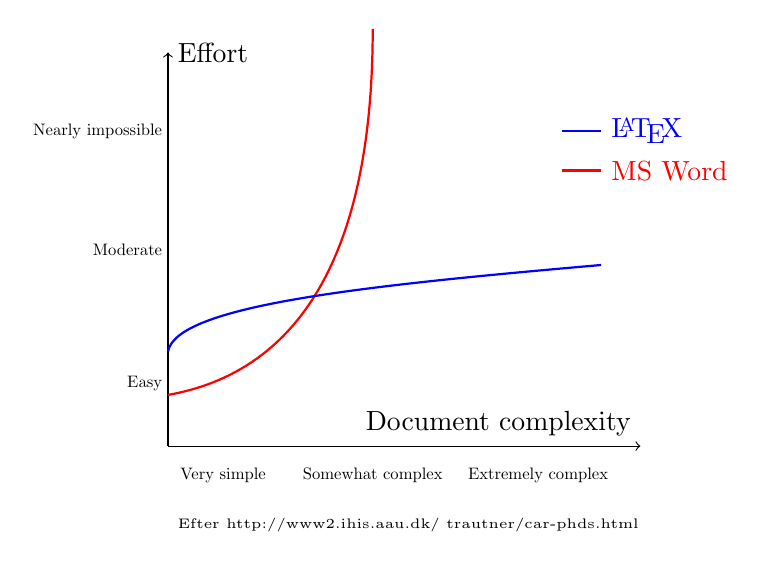
\begin{tikzpicture}
%\draw[step=0.2cm] (0, 0) grid (4, 4);
%\draw node[anchor=south west, xshift=-0.87cm, yshift=-0.88cm, opacity=0.5] {\includegraphics[width=8cm]{learningcurve.jpg}};
\draw[->] (0, 0) -- (0, 5) node[right] {Effort};
\draw[->] (0, 0) -- (6, 0) node[above left] {Document complexity};
\draw[thick, red] (0, 0.65) .. controls +(10: 1.6cm) and +(270: 3cm) .. (2.6, 5.3);
\draw[thick, blue] (0, 1.2) .. controls +(80: 0.6cm) and +(185: 3cm) .. (5.5, 2.30);
\draw (0, 0.8) node[left, scale=0.6] {Easy};
\draw (0, 2.5) node[left, scale=0.6] {Moderate};
\draw (0, 4.0) node[left, scale=0.6] {Nearly impossible};
\draw (0.7, 0) node[below=0.2cm, scale=0.6] {Very simple};
\draw (2.6, 0) node[below=0.2cm, scale=0.6] {Somewhat complex};
\draw (4.7, 0) node[below=0.2cm, scale=0.6] {Extremely complex};
\draw[thick, blue] (5, 4) -- (5.5, 4) node[right] {\LaTeX};
\draw[thick, red] (5, 3.5) -- (5.5, 3.5) node[right] {MS Word};
\draw (0, -1) node[right] {\tiny Efter \url{http://www2.ihis.aau.dk/~trautner/car-phds.html}};
\end{tikzpicture}

}


% ================================================================
\subsection{Programmer}
\frame
{
	\frametitle{Hvilke programmer skal jeg bruge?}
	Oversættere (oversætter et latex dokument til f.eks. en pdf fil)
	\begin{itemize}
		\item MiKTeX, \\
			{\tiny \url{http://miktex.org/2.9/setup}}
	\end{itemize}

	Editorer (det program du bruger til at rette i latex dokumenter)
	\begin{itemize}
		\item	TeXworks, \\
			{\tiny \url{http://www.tug.org/texworks/}}
		\item	TexnicCenter, \\
			{\tiny \url{http://www.texniccenter.org/}}
		\item 	Texmaker, \\
			{\tiny \url{http://www.xm1math.net/texmaker/}}
	\end{itemize}
}

% ================================================================
%\subsection{Ekstra scripts til TeXworks}
\frame
{
	\frametitle{Ekstra scripts til TeXworks}

	\begin{itemize}
	\item Hjælp til at finde fejl i latex dokumenter \\
		{\tiny \url{https://github.com/henrikmidtiby/TeXworks-scripts/tree/master/latexErrors}}
	\item Autocompletion \\
		{\tiny \url{https://github.com/henrikmidtiby/TeXworks-scripts/tree/master/autocomplete}}
	\end{itemize}
}


% ================================================================
\frame
{
\frametitle{TeXworks}
	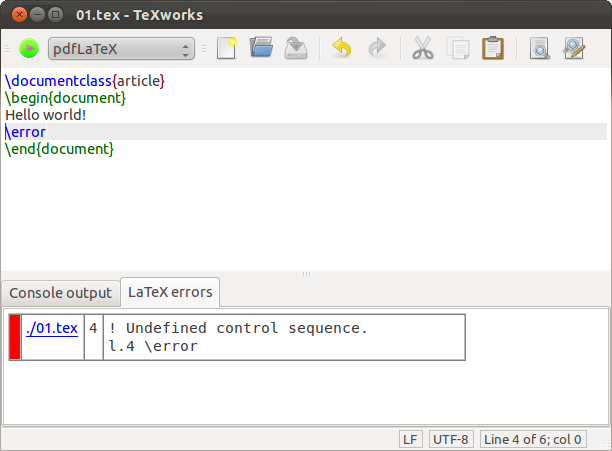
\includegraphics[height=6cm]{pic/texworksLatexErrors.png}
}

% ================================================================
% ================================================================
\section{Eksempler 1}
\frame{
\begin{multicols}{2}
	\tableofcontents[currentsection] 
\end{multicols} 
}

% ================================================================
\subsection{Minimalt eksempel}
\frame
{
	\frametitle{Minimalt eksempel}
	\lstinputlisting{examples/01.tex}
}

\frame
{
	\insertPDF{examples/01.pdf}
}


% ================================================================
\subsection{Danske tegn}
\begin{frame}[fragile]
	\frametitle{Danske tegn -- Problemer}

\begin{verbatim}
\documentclass{article}
\begin{document}
Hello world!

På Ærø ligger Marstal.
\end{document}
\end{verbatim}

\end{frame}
\frame
{
	\insertPDF{examples/01b.pdf}
}


\begin{frame}[fragile]
	\frametitle{Danske tegn -- Problemet løst}

\begin{verbatim}
\documentclass{article}
\usepackage[utf8]{inputenc}
\begin{document}
Hello world!

På Ærø ligger Marstal.
\end{document}
\end{verbatim}

\end{frame}
\frame
{
	\insertPDF{examples/01c.pdf}
}






% ================================================================
\subsection{Afsnit}
\frame
{
	\frametitle{Afsnit}
	\lstinputlisting{examples/02paragraphs.tex}
}

\frame
{
	\insertPDF{examples/02paragraphs.pdf}
}

% ================================================================
\subsection{Indholdsfortegnelse}
\frame
{
	\frametitle{Indholdsfortegnelse}
	\lstinputlisting{examples/02.tex}
}

\frame
{
	\insertPDF{examples/02firstRun.pdf}
	\addnote{For at opdatere indholdet i indholdsfortegnelsen er det nødvendigt at oversætte filen to gange.}
}

\frame
{
	\insertPDF{examples/02.pdf}
}


% ================================================================
%\subsection{Informationsflow}
\frame
{
	\frametitle{Kompilering og informationsflow}
	
	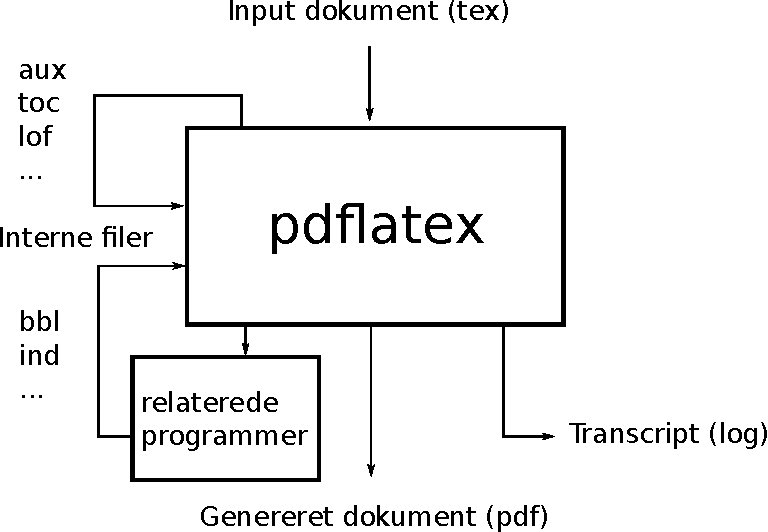
\includegraphics[width=8cm]{pic/latexInformationFlow.pdf}
	
	\source{Efter figur 1.1 i Latex Companion.}

}


% Der er problemer med at indsætte æøå vha. listingspakken
%\frame
%{
%	\frametitle{ÆØÅ problemer}
%	\lstinputlisting[extendedchars]{examples/03.tex}
%}
%
%\frame
%{
%	\insertPDF{examples/03.pdf}
%}

% ================================================================
\subsection{Referencer}
\frame {
	\frametitle{Referencer}
	\lstinputlisting[firstline=4, lastline=18]{examples/05.tex}
}

\frame {
	\insertPDF{examples/05firstRun.pdf}
	\addnote{Henvisninger til referencer kræver også to oversættelser.}
}

\frame {
	\insertPDF{examples/05.pdf}
}


% ================================================================
\subsection{Kommando anatomi}
\frame {
	\frametitle{Kommando anatomi}
	Generel opbygning
	\lstinputlisting[firstline=1, lastline=5]{commandanatomy.tex}
	Eksempler
	\lstinputlisting[firstline=6, lastline=9]{commandanatomy.tex}
}


% ================================================================
% ================================================================
\section{Eksempler 2}
\frame{
\begin{multicols}{2}
	\tableofcontents[currentsection] 
\end{multicols} 
}

% ================================================================
\subsection{Lister}
\frame {
	\frametitle{Lister}
	\lstinputlisting[firstline=5, lastline=18]{examples/04.tex}
}

\frame {
	\insertPDF{examples/04.pdf}
}

% ================================================================
\subsection{Lister i lister}
\frame {
	\frametitle{Lister i lister}
	\lstinputlisting[firstline=5, lastline=12]{examples/04b.tex}
}

\frame {
	\insertPDF{examples/04b.pdf}
}

% ================================================================
\subsection{Tabeller}
\frame {
	\frametitle{Tabeller}
	\lstinputlisting[firstline=5, lastline=18]{examples/10.tex}
}

\frame {
	\insertPDF{examples/10.pdf}
}


% ================================================================
\subsection{Figurer}
\frame {
	\frametitle{Figurer}
	\lstinputlisting{examples/06.tex}
}

\frame {
	\insertPDF{examples/06.pdf}
}


\frame{
	\frametitle{Ide til en mappestruktur}
	
	Mappe struktur for et latex dokument (undermapper til billeder m.m.)
	\begin{itemize}
		\item	project.tex
		\item	pic
		\begin{itemize}
			\item	vandstraaler.jpg
		\end{itemize}
	\end{itemize}

}


% ================================================================
\subsection{Formler}
\begin{frame}[fragile]
	\frametitle{Formler 0}
	{\Huge
	\begin{align*}
		\frac{a}{b}	\qquad a^b	\qquad \theta
	\end{align*}
	}
	\pause
	\begin{verbatim}
\frac{a}{b}
a^b
\theta
	\end{verbatim}
\end{frame}


\frame {
	\frametitle{Formler I}
	\lstinputlisting[firstline=2, lastline=2, basicstyle=\color{red}]{examples/07a.tex}
	\lstinputlisting[firstline=4, lastline=14]{examples/07a.tex}
}

\frame {
	\insertPDF{examples/07a.pdf}
}


\frame {
	\frametitle{Hvor finder man symbolerne?}

	\begin{itemize}
	\item Detexify, \\
			{\tiny \url{http://detexify.kirelabs.org/classify.html}}
	\item The Comprehensive LaTeX Symbol List, \\
			{\tiny \url{http://www.ctan.org/tex-archive/info/symbols/comprehensive/symbols-a4.pdf}}
	\end{itemize}
	
	\centering	
	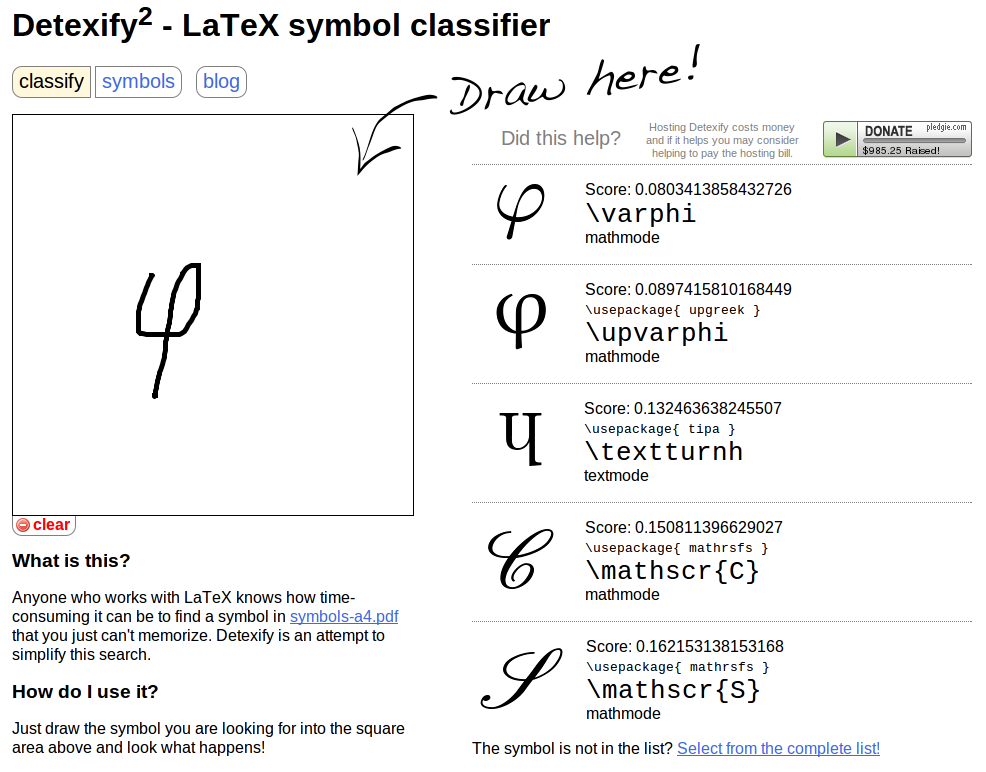
\includegraphics[width=7cm]{pic/detexify.png}
}

\frame {
	\frametitle{Tegn formlerne!}

	\begin{itemize}
	\item MyScript MathPad, \\
			{\tiny \url{https://itunes.apple.com/app/myscript-mathpad/id674996719}}
	\end{itemize}
	
	\centering	
	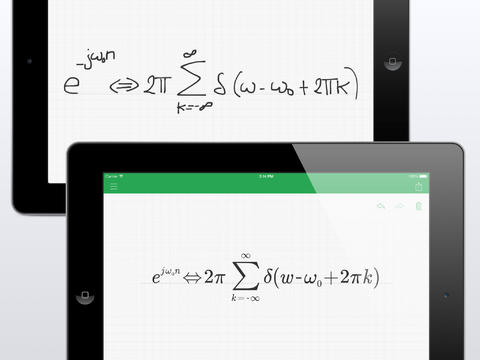
\includegraphics[width=7cm]{pic/myscriptmathpad.jpg}
}



\frame {
	\frametitle{Formler II}
	\lstinputlisting{examples/07.tex}
}

\frame {
	\insertPDF{examples/07.pdf}
	\lstinputlisting[firstline=2, lastline=2, basicstyle=\color{red}]{examples/07.tex}
	\lstinputlisting[firstline=4, lastline=13]{examples/07.tex}
}



% ================================================================
\subsection{Miljø anatomi}
\frame {
	\frametitle{Miljø (environment) anatomi}
	Generel opbygning
	\lstinputlisting[firstline=1, lastline=5]{environmentanatomy.tex}
	Eksempler
	\lstinputlisting[firstline=6]{environmentanatomy.tex}
}


% ================================================================
\subsection{Fejlsøgning}
\frame {
	\frametitle{Fejlsøgning}

	Der er eksempler på forskellige fejl i errors mappen.

	Kan I finde og rette disse fejl?


	Strategi: 
	\begin{itemize}
	\item Binær søgning ved at placere \textbackslash{}end\{document\} forskellige steder i dokumentet
	\item Udkommentere enkelte linjer
	\end{itemize}
}





% ================================================================
% ================================================================
\section{Eksempler 3}
\frame{
\begin{multicols}{2}
	\tableofcontents[currentsection] 
\end{multicols} 
}

% ================================================================
\subsection{Cite and bibitem}
\frame {
	\frametitle{Cite and bibitem}
	\lstinputlisting[firstline=4, lastline=20]{examples/08.tex}
}

\frame {
	\insertPDF{examples/08firstRun.pdf}
}

\frame {
	\insertPDF{examples/08.pdf}
}

%}


% ================================================================
\subsection{Bibtex}


\frame {
	\frametitle{Bibtex I}
	\lstinputlisting{examples/09.tex}
}

\frame {
	\frametitle{Bibtex II (bibtexfile.bib)}
	\lstinputlisting{examples/bibtexfile.bib}
}

\frame {
	\insertPDF{examples/09firstRun.pdf}
}

\frame {
	\insertPDF{examples/09.pdf}
}


\frame
{
	\frametitle{Bibtex og informationsflow}
	
	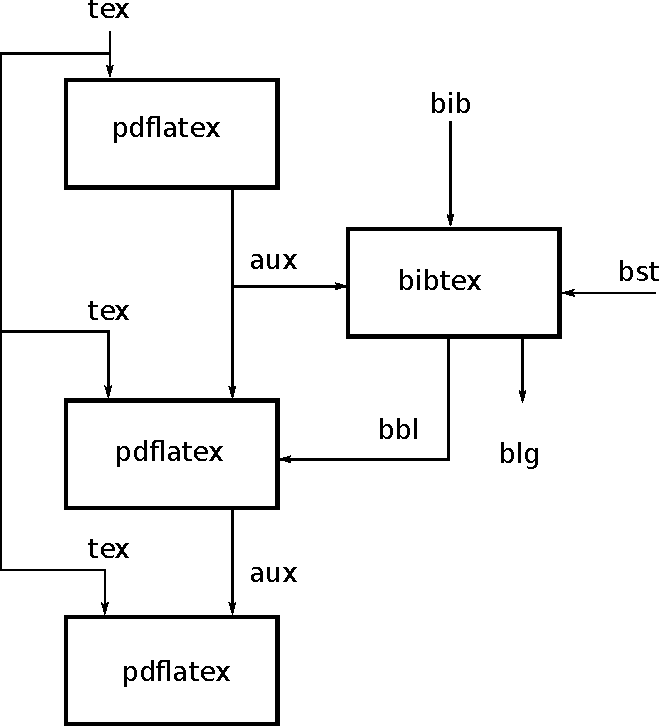
\includegraphics[width=5.8cm]{pic/bibtexInformationFlow.pdf}
	\source{Efter figur 12.1 i Latex Companion.}
}


\frame
{
	\frametitle{Jabref}
	
	\centering
	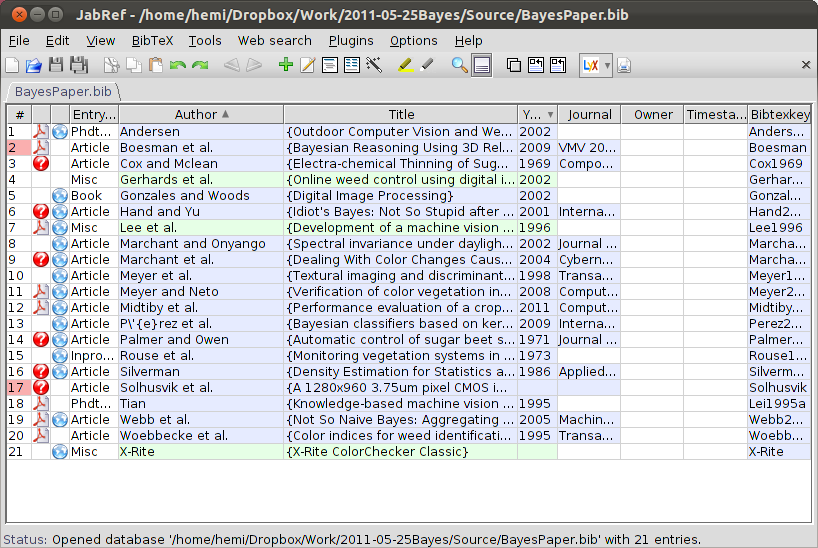
\includegraphics[width=9cm]{pic/jabref.png}

	{\tiny \url{http://jabref.sourceforge.net/}}
}

\frame
{
	\frametitle{Mendeley}

	\centering
	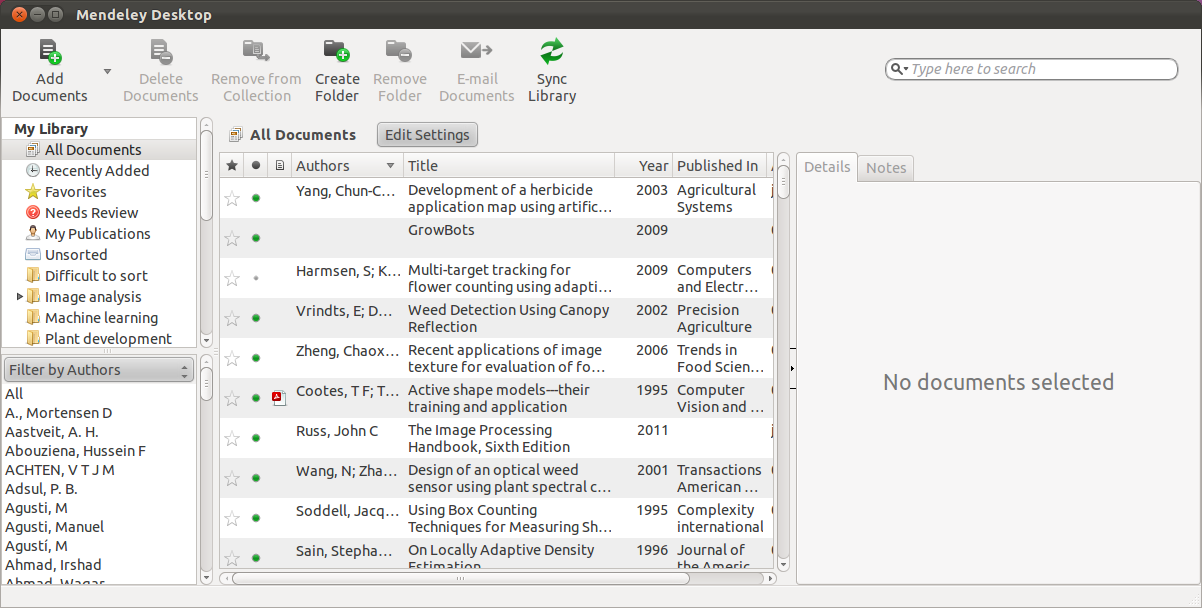
\includegraphics[width=9cm]{pic/mendeley.png}

	{\tiny \url{http://www.mendeley.com/}}
}


% ================================================================
\subsection{Todonotes}

\frame {
	\frametitle{Todonotes}
	\lstinputlisting[firstline=2, lastline=2, basicstyle=\color{red}]{examples/11.tex}
	\lstinputlisting[firstline=5, lastline=15]{examples/11.tex}
}

\frame {
	\insertPDF[0.6]{examples/11.pdf}
}


% ================================================================
\subsection{Tikz}

\frame {
	\frametitle{Tikz}
	\lstinputlisting[firstline=2, lastline=2, basicstyle=\color{red}\footnotesize]{examples/12.tex}
	\lstinputlisting[firstline=4, lastline=18, basicstyle=\footnotesize]{examples/12.tex}
}

\frame {
	\insertPDF[0.6]{examples/12.pdf}
}


% ================================================================
\subsection{mhchem}

\frame {
	\frametitle{mhchem (1/2)}
	\lstinputlisting[firstline=2, lastline=2, basicstyle=\color{red}\footnotesize]{examples/13mhchem.tex}
	\lstinputlisting[firstline=4, lastline=18, basicstyle=\footnotesize]{examples/13mhchem.tex}
}

\frame {
	\insertPDF[0.6]{examples/13mhchem.pdf}
}

\frame {
	\frametitle{mhchem (2/2)}
	\lstinputlisting[firstline=5, lastline=10, basicstyle=\footnotesize]{examples/13mhchemReactions.tex}
}

\frame {
	\insertPDF[0.6]{examples/13mhchemReactions.pdf}
}

% ================================================================
\subsection{siunitx}

\frame {
	\frametitle{siunitx}
	\lstinputlisting[firstline=2, lastline=2, basicstyle=\color{red}\footnotesize]{examples/14siunitx.tex}
	\lstinputlisting[firstline=4, lastline=14, basicstyle=\footnotesize]{examples/14siunitx.tex}
}

\frame {
	\insertPDF[0.6]{examples/14siunitx.pdf}
}


% ================================================================
\subsection{hyperref}

\frame {
	\frametitle{hyperref}
	\lstinputlisting[firstline=2, lastline=3, basicstyle=\color{red}\footnotesize]{examples/15hyperref.tex}
	\lstinputlisting[firstline=5, lastline=14, basicstyle=\footnotesize]{examples/15hyperref.tex}
}

\frame {
	\insertPDF[0.6]{examples/15hyperreffirstRun.pdf}
}

\frame {
	\insertPDF[0.6]{examples/15hyperref.pdf}
}


% ================================================================
\subsection{include / input}

\frame {
	\frametitle{include / input}
	16include.tex
	\lstinputlisting[firstline=1, lastline=4, basicstyle=\footnotesize]{examples/16include.tex}
	
	\vspace{1cm}
	16includePartA.tex
	\lstinputlisting[firstline=1, lastline=2, basicstyle=\footnotesize]{examples/16includePartA.tex}
}

\frame {
	\insertPDF[0.6]{examples/16include.pdf}
}


% ================================================================
% ================================================================
\section{En rapport skabelon}
\frame{
\begin{multicols}{2}
	\tableofcontents[currentsection] 
\end{multicols} 
}


%\frame {
%	\frametitle{Rapport skabelon}
%	\lstinputlisting[firstline=1, lastline=14]{examples/skabelon/doc/project.tex}
%}

{
% The following line is needed to avoid beamer 
% placing a white background on top of the other contents
\setbeamercolor{background canvas}{bg=}
\includepdf[pages={1, 2, 3, 4, 5, 6}, nup=2x1, frame, delta=0.5cm 0.5cm, scale=0.9]
	{examples/skabelon/doc/project.pdf}
}



% ================================================================
% ================================================================
\section{Ressourcer / Læsestof}
\frame {
	\begin{itemize}
	\item	The not so short introduction to latex 	\\
			{\tiny \url{http://www.ctan.org/tex-archive/info/lshort/english/lshort.pdf}}
	\item	Introduktion til \LaTeX 				\\
			{\tiny \url{http://imf.au.dk/system/latex/bog/}}
	\item	Den nye LaTeX for forfattere \\
			{\tiny \url{http://dirac.ruc.dk/imfufalatex/ltxnoterh.pdf}}
	\item	Bog om latex på wikibooks 				\\
			{\tiny \url{http://en.wikibooks.org/wiki/LaTeX}}
	\item	The \LaTeX{} companion					\\
			Meget grundig bog om latex
	\end{itemize}
}


\frame{
	\frametitle{Andre tips}
	Hvis latex kompileringen fejler kan problemet nogle gange løses ved at slette
	alle \emph{.aux} filer.
}


\end{document}
